\chapter{Appendix A:\newline Code Documentation}
\label{apx:Code}

The code documentation aims to describe the overall structure of our implementation as well as the main functions of our PHP and JavaScript code. We first provide a general overview of the code structure, before going into more code specific details. 

\section{Structure}
\label{sec:CodeStructure}
When creating a comprehensive website it is important to create a code and document structure that clearly separates the different modules. These modules were in our case: backend code, JavaScript code, style code, markup code and image files. The backend code written in PHP is divided into three categories: documents performing database queries, documents creating forms or pages that are fetched using AJAX and lastly documents with general functions for images, sharing and login. The JavaScript code consists mostly of functions performed when a page is loaded or when the user interacts with a page. This can be through mouse events or typing text. The style code is a collection of CSS documents used to style the different HTML elements, such as divs, buttons and text fields. All image files are separated from the code documents and placed in their own folder. In figure \ref{fig:CodeStructureStruc} the overall structure can be seen.

\begin{figure}[ht!]
  \centering
  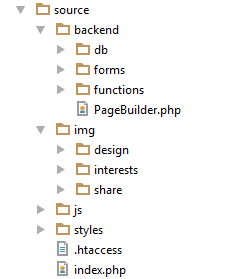
\includegraphics[width=50mm]{./Appendix/CodeDocumentation/img/structure}
  \caption{Overall structure of the code.}
  \label{fig:CodeStructureStruc}
\end{figure}

\section{Details}
\label{sec:CodeDetails}

\subsection{Backend/DB}
\label{subsec:CodeDetailsBackendDB}

\subsubsection{DBComments}
\begin{minipage}{\linewidth}
  \centering
  \setlength{\tabcolsep}{12pt}
  \rowcolors{1}{blue!20}{blue!10}
  \begin{tabular}{|p{0.35\linewidth}|p{0.55\linewidth}|}
  \hline
  \cellcolor{gray!25} Function & \cellcolor{gray!25} Description \\
  \hline
  getComments(threadID) & Fetches all comments related to a \textit{threadID} from the database. \\
  insertComment(threadID, parent, username, comment) & Inserts a new comment into the database. All comments have a creator (\textit{username}), a \textit{threadID} and the \textit{comment} itself. If the comment is a reply, it also has a \textit{parent} comment. \\
  \hline  
  \end{tabular}
\end{minipage}

\subsubsection{DBEvents}
\begin{minipage}{\linewidth}
  \centering
  \setlength{\tabcolsep}{12pt}
  \rowcolors{1}{blue!20}{blue!10}
  \begin{tabular}{|p{0.35\linewidth}|p{0.55\linewidth}|}
  \hline
  \cellcolor{gray!25} Function & \cellcolor{gray!25} Description \\
  \hline
  addEvent(username, title, description, interests, coordinates, numPeople, time) & Validates and inserts a new event into the database. All events have a creator(\textit{username}), a string \textit{title} and \textit{description}, max number of people and \textit{time} (unix timestamp). Additionally they are tagged with \textit{interests} and geographical \textit{coordinates}. \\
  fetchEvent(eventID) & Fetches an event based on the \textit{eventID}. \\
  voteEvent(eventID, up, down) & Adds \textit{up} number of positive votes and \textit{down} number of negative votes to an \textit{eventID}. \\
  searchEvents(interests, bounds, page) & Fetches a \textit{page} of events matching tagged under \textit{interests} within a geographical \textit{bound}. \\
  \hline  
  \end{tabular}
\end{minipage}

\subsubsection{DBInterests}
\begin{minipage}{\linewidth}
  \centering
  \setlength{\tabcolsep}{12pt}
  \rowcolors{1}{blue!20}{blue!10}
  \begin{tabular}{|p{0.35\linewidth}|p{0.55\linewidth}|}
  \hline
  \cellcolor{gray!25} Function & \cellcolor{gray!25} Description \\
  \hline
  getInterest(id) & Fetches the interest with the given \textit{id}. \\
  HTTP GET interest & Returns a JSON array of interests that begin with \textit{interest}. \\
  \hline  
  \end{tabular}
\end{minipage}

\subsubsection{DBPhotos}
\begin{minipage}{\linewidth}
  \centering
  \setlength{\tabcolsep}{12pt}
  \rowcolors{1}{blue!20}{blue!10}
  \begin{tabular}{|p{0.35\linewidth}|p{0.55\linewidth}|}
  \hline
  \cellcolor{gray!25} Function & \cellcolor{gray!25} Description \\
  \hline
  addPhoto(uploader, title, coordinates, interests, description) & Validates and inserts a new photo into the database. All photos have an \textit{uploader}, a string \textit{title} and \textit{description}. Additionally they are tagged with \textit{interests} and geographical \textit{coordinates}. \\
  removePhoto(id) & Removes a photo from the database based on the photo \textit{id}. \\
  getPhotoDetails(id) & Fetches all data of a photo based on the photo \textit{id}. \\
  votePhoto(photoID, up, down) & Adds \textit{up} number of positive votes and \textit{down} number of negative votes to a \textit{photoID}. \\
  searchPhotos(interests, bounds, page) & Fetches a \textit{page} of photos matching tagged \textit{interests} within a geographical \textit{bound}. \\
  \hline  
  \end{tabular}
\end{minipage}

\subsubsection{DBUsers}
\begin{minipage}{\linewidth}
  \centering
  \setlength{\tabcolsep}{12pt}
  \rowcolors{1}{blue!20}{blue!10}
  \begin{tabular}{|p{0.35\linewidth}|p{0.55\linewidth}|}
  \hline
  \cellcolor{gray!25} Function & \cellcolor{gray!25} Description \\
  \hline
  addUser(username, password, first name, last name, gender) & Validates and inserts a new user into the database. All users have a \textit{username} and a \textit{password}, as well as a \textit{first name}, a \textit{last name} and a \textit{gender}. \\
  checkLogin(username, password) & Checks if the \textit{password} matches the given \textit{username}. \\
  usernameExists(username) & Returns true if a \textit{username} is already taken. \\
  \hline  
  \end{tabular}
\end{minipage}

\subsubsection{DBVotes}
\begin{minipage}{\linewidth}
  \centering
  \setlength{\tabcolsep}{12pt}
  \rowcolors{1}{blue!20}{blue!10}
  \begin{tabular}{|p{0.35\linewidth}|p{0.55\linewidth}|}
  \hline
  \cellcolor{gray!25} Function & \cellcolor{gray!25} Description \\
  \hline
  registerVote(contentID, vote) & Registers that the logged in user has voted \textit{vote} on \textit{contentID}. \\
  didVote(contentID) & Returns whether the logged in user has voted on \textit{contentID}. \\
  \hline  
  \end{tabular}
\end{minipage}

\subsection{Backend/Forms}
\label{subsec:CodeDetailsBackendForms}

\subsubsection{CommentForm}
\begin{minipage}{\linewidth}
  \centering
  \setlength{\tabcolsep}{12pt}
  \rowcolors{1}{blue!20}{blue!10}
  \begin{tabular}{|p{0.35\linewidth}|p{0.55\linewidth}|}
  \hline
  \cellcolor{gray!25} Function & \cellcolor{gray!25} Description \\
  \hline
  getCommentsForm(id) & Returns the full markup for the comment section for thread \textit{id}. \\
  showComment(comments) & Creates the comment thread layout for current and all nested comments inside \textit{comments} array. \\
  \hline
  \end{tabular}
\end{minipage}

\subsubsection{EventForm}
\begin{minipage}{\linewidth}
  \centering
  \setlength{\tabcolsep}{12pt}
  \rowcolors{1}{blue!20}{blue!10}
  \begin{tabular}{|p{0.35\linewidth}|p{0.55\linewidth}|}
  \hline
  \cellcolor{gray!25} Function & \cellcolor{gray!25} Description \\
  \hline
  HTTP POST & Passes on HTTP POST variables to \textit{DBEvent.addEvent()}, returns JSON a formatted response. \\
  HTTP GET & Returns HTML for event creation form. \\
  \hline
  \end{tabular}
\end{minipage}

\subsubsection{GetLocation}
\begin{minipage}{\linewidth}
  \centering
  \setlength{\tabcolsep}{12pt}
  \rowcolors{1}{blue!20}{blue!10}
  \begin{tabular}{|p{0.35\linewidth}|p{0.55\linewidth}|}
  \hline
  \cellcolor{gray!25} Function & \cellcolor{gray!25} Description \\
  \hline
  HTTP POST image & Checks if \textit{image} has EXIF GPS coordinates attached to it. \\
  \hline
  \end{tabular}
\end{minipage}

\subsubsection{LogForm}
\begin{minipage}{\linewidth}
  \centering
  \setlength{\tabcolsep}{12pt}
  \rowcolors{1}{blue!20}{blue!10}
  \begin{tabular}{|p{0.35\linewidth}|p{0.55\linewidth}|}
  \hline
  \cellcolor{gray!25} Function & \cellcolor{gray!25} Description \\
  \hline
  HTTP POST & Passes on HTTP POST variables to \textit{DBUsers.checkLogin()}, returns JSON a formatted response. \\
  HTTP GET & Returns HTML for login form. \\
  \hline
  \end{tabular}
\end{minipage}

\subsubsection{MapLookup}
\begin{minipage}{\linewidth}
  \centering
  \setlength{\tabcolsep}{12pt}
  \rowcolors{1}{blue!20}{blue!10}
  \begin{tabular}{|p{0.35\linewidth}|p{0.55\linewidth}|}
  \hline
  \cellcolor{gray!25} Function & \cellcolor{gray!25} Description \\
  \hline
  HTTP GET & Creates a page with Google Maps location autocomplete and Google Maps map. Is meant to be opened in a separate window and used as a location selector: on window close, it returns the selected location. \\
  \hline
  \end{tabular}
\end{minipage}

\subsubsection{OverlayEvents}
\begin{minipage}{\linewidth}
  \centering
  \setlength{\tabcolsep}{12pt}
  \rowcolors{1}{blue!20}{blue!10}
  \begin{tabular}{|p{0.35\linewidth}|p{0.55\linewidth}|}
  \hline
  \cellcolor{gray!25} Function & \cellcolor{gray!25} Description \\
  \hline
  HTTP GET id & Returns HTML for the overlay with event details, comments and sharing for event \textit{id}. \\
  \hline
  \end{tabular}
\end{minipage}

\subsubsection{OverlayPhotos}
\begin{minipage}{\linewidth}
  \centering
  \setlength{\tabcolsep}{12pt}
  \rowcolors{1}{blue!20}{blue!10}
  \begin{tabular}{|p{0.35\linewidth}|p{0.55\linewidth}|}
  \hline
  \cellcolor{gray!25} Function & \cellcolor{gray!25} Description \\
  \hline
  HTTP GET id & Returns HTML for the overlay with photo details, comments and sharing for photo \textit{id}. \\
  \hline
  \end{tabular}
\end{minipage}

\subsubsection{RegForm}
\begin{minipage}{\linewidth}
  \centering
  \setlength{\tabcolsep}{12pt}
  \rowcolors{1}{blue!20}{blue!10}
  \begin{tabular}{|p{0.35\linewidth}|p{0.55\linewidth}|}
  \hline
  \cellcolor{gray!25} Function & \cellcolor{gray!25} Description \\
  \hline
  HTTP POST & Passes on HTTP POST variables to \textit{DBUsers.addUser()}, returns JSON a formatted response. \\
  HTTP GET & Returns HTML for register form. \\
  \hline
  \end{tabular}
\end{minipage}

\subsubsection{UploadPhoto}
\begin{minipage}{\linewidth}
  \centering
  \setlength{\tabcolsep}{12pt}
  \rowcolors{1}{blue!20}{blue!10}
  \begin{tabular}{|p{0.35\linewidth}|p{0.55\linewidth}|}
  \hline
  \cellcolor{gray!25} Function & \cellcolor{gray!25} Description \\
  \hline
  uploadImage(title, interests, description, image, coordinates) & Validates and scales an image before inserting it into the database via \textit{DBPhotos.addPhoto()}. \\
  HTTP GET & Returns HTML for upload image form. \\
  HTTP POST & Passes on HTTP POST variables to \textit{uploadImage()}, returns JSON a formatted response. \\
  \hline
  \end{tabular}
\end{minipage}

\subsubsection{VoteForm}
\begin{minipage}{\linewidth}
  \centering
  \setlength{\tabcolsep}{12pt}
  \rowcolors{1}{blue!20}{blue!10}
  \begin{tabular}{|p{0.35\linewidth}|p{0.55\linewidth}|}
  \hline
  \cellcolor{gray!25} Function & \cellcolor{gray!25} Description \\
  \hline
  getVoter(database, id, up, down) & Returns HTML for voting from for an item \textit{id} in \textit{database} with \textit{up} number of positive and \textit{down} number of negative votes. \\
  HTTP GET & Passes on HTTP GET variables to \textit{DBVotes.registerVote()}, returns \textit{getVoter()} form. \\
  \hline
  \end{tabular}
\end{minipage}

\subsection{Backend/Functions}
\label{subsec:CodeDetailsBackendFunctions}

\subsubsection{Image}
\begin{minipage}{\linewidth}
  \centering
  \setlength{\tabcolsep}{12pt}
  \rowcolors{1}{blue!20}{blue!10}
  \begin{tabular}{|p{0.35\linewidth}|p{0.55\linewidth}|}
  \hline
  \cellcolor{gray!25} Function & \cellcolor{gray!25} Description \\
  \hline
  scaleImage(image, maxWidth, maxHeight, path) & Scales \textit{image} to fit inside \textit{maxWidth} x \textit{maxHeight}. Saves the result in \textit{path}. \\
  getEXIFGPS(image) & Returns coordinates stored in under EXIF GPS tag inside \textit{image}. \\
  \hline
  \end{tabular}
\end{minipage}

\subsubsection{Log}
\begin{minipage}{\linewidth}
  \centering
  \setlength{\tabcolsep}{12pt}
  \rowcolors{1}{blue!20}{blue!10}
  \begin{tabular}{|p{0.35\linewidth}|p{0.55\linewidth}|}
  \hline
  \cellcolor{gray!25} Function & \cellcolor{gray!25} Description \\
  \hline
  login(username, password) & Checks if \textit{password} matches the given \textit{username}. If matching, the user is signed in. \\
  loginPlainText(username, password) & Hashes the plaintext \textit{password} and calls \textit{login()}. \\
  logout() & The current user is signed out. \\
  isLoggedIn() & Checks if user is signed in. \\
  HTTP GET out & Calls \textit{logout()}. \\
  \hline
  \end{tabular}
\end{minipage}

\subsubsection{Sharing}
\begin{minipage}{\linewidth}
  \centering
  \setlength{\tabcolsep}{12pt}
  \rowcolors{1}{blue!20}{blue!10}
  \begin{tabular}{|p{0.35\linewidth}|p{0.55\linewidth}|}
  \hline
  \cellcolor{gray!25} Function & \cellcolor{gray!25} Description \\
  \hline
  getShareButtons(url, title, description) & Returns HTML sharing buttons for \textit{url}, with \textit{title} and a \textit{description}. \\
  \hline
  \end{tabular}
\end{minipage}

\subsubsection{Time}
\begin{minipage}{\linewidth}
  \centering
  \setlength{\tabcolsep}{12pt}
  \rowcolors{1}{blue!20}{blue!10}
  \begin{tabular}{|p{0.35\linewidth}|p{0.55\linewidth}|}
  \hline
  \cellcolor{gray!25} Function & \cellcolor{gray!25} Description \\
  \hline
  unixTimeToStringDate(time) & Converts Unix \textit{time} to the format (DD MM YYYY). \\
  \hline
  \end{tabular}
\end{minipage}

\subsection{JavaScript}
\label{subsec:CodeDetailsJavaScript}

\subsubsection{2DSearch}
\begin{minipage}{\linewidth}
  \centering
  \setlength{\tabcolsep}{12pt}
  \rowcolors{1}{blue!20}{blue!10}
  \begin{tabular}{|p{0.35\linewidth}|p{0.55\linewidth}|}
  \hline
  \cellcolor{gray!25} Function & \cellcolor{gray!25} Description \\
  \hline
  initializeGMaps() & Creates a Google Maps map, Google Maps places autocomplete and creates events listeners to call \textit{doSearch()}. \\
  initializeTokenAutoComplete() & Initializes jQuery Tokeninput with event listeners to call \textit{doSearch()}. \\
  initializePageListeners() & Initializes other page listeners, such as mouse scroll listeners to load more elements and click listeners to display the overlay with expanded view. \\
  doSearch(append) & Performs a search with the currently selected interests, bounds and database. If \textit{append} is set, the result will be appended to the bottom, otherwise all previous results will be replaced with new result. \\
  vote(vote, contentID, database) & Sends AJAX request to register \textit{vote} on \textit{contentID} in \textit{database}. \\
  \hline
  \end{tabular}
\end{minipage}

\subsubsection{Comment}
\begin{minipage}{\linewidth}
  \centering
  \setlength{\tabcolsep}{12pt}
  \rowcolors{1}{blue!20}{blue!10}
  \begin{tabular}{|p{0.35\linewidth}|p{0.55\linewidth}|}
  \hline
  \cellcolor{gray!25} Function & \cellcolor{gray!25} Description \\
  \hline
  addComment(where, parent) & Adds a HTML form to \textit{where} with \textit{parent} id. \\
  addSubmit(from, parent) & Sends AJAX request to post a comment with \textit{parent} id that is closest to \textit{from}. \\
  \hline
  \end{tabular}
\end{minipage}

\section{JavaScript Libraries used}
\begin{itemize}
  \item Google Maps JavaScript API v3 (\cite{website:maps-api-js})
  \begin{itemize}
    \item MarkerClusterer (\cite{website:maps-clusterer})
  \end{itemize}
  \item jQuery 1.11.1 (\cite{website:jquery})
  \begin{itemize}
    \item DateTimePicker 2.3.7 (\cite{website:datetime})
    \item Tokeninput (\cite{website:tokeninput})
    \item Modal (\cite{website:modal})
  \end{itemize}
\end{itemize}